\begin{center}
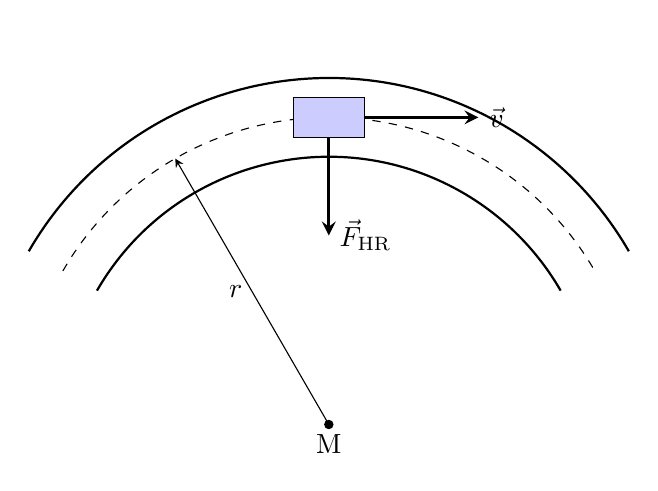
\begin{tikzpicture}[>=stealth]
 \draw[thick] (0,0) ++(150:4.4) arc (150:30:4.4);
 \draw[thick] (0,0) ++(150:3.4) arc (150:30:3.4);
 \draw[dashed] (0,0) ++(150:3.9) arc (150:30:3.9);
 \fill (0,0) circle (0.06) node[below] {M};
 \draw[->] (0,0) -- (120:3.9) node[pos=0.5, left] {$r$};
 \fill[blue!20] (-0.45,3.65) rectangle (0.45,4.15);
 \draw (-0.45,3.65) rectangle (0.45,4.15);
 \draw[->, very thick] (0.45,3.9) -- (1.9,3.9) node[right] {$\vec v$};
 \draw[->, very thick] (0,3.65) -- (0,2.4) node[right] {$\vec F_\mathrm{HR}$};
\end{tikzpicture}
\end{center}

Auf ebener Strasse liefert allein die Haftreibungskraft zwischen Reifen und Strasse die Zentripetalkraft (Draufsicht). Sie kann höchstens $F_\mathrm{HR} = \mu_\mathrm{H}\,F_\mathrm{N} = \mu_\mathrm{H}\,m\,g$ betragen. Für Pneus auf trockener Asphaltstrasse ist $\mu_\mathrm{H} = \muKuO$ (FoTaBe S.~189). Die Zentripetalbedingung lautet
\begin{align}
 \frac{m\,v^2}{r} &= \mu_\mathrm{H}\,m\,g
\end{align}
Die Masse kürzt sich, und für die Höchstgeschwindigkeit folgt
\begin{align}
 v &= \vKuF \\
   &= \sqrt{\muKu\cdot\gE\cdot\rKu} \\
   &= \vKu \approx \result{\vKuP{0}{2}} = \vKukP{0}{3}
\end{align}
Da $\mu_\mathrm{H}$ je nach Belag und Reifen schwankt, ist das nur ein Richtwert.
